\documentclass[12pt]{article}
\usepackage{listings}
\usepackage{color}
\usepackage{graphicx}
\usepackage{float}
\usepackage{hyperref}
\usepackage[many]{tcolorbox}
\usepackage[colorinlistoftodos]{todonotes}
\usepackage[utf8]{inputenc}
\usepackage{tikz}
\usepackage{pgfplots}
\usepgfplotslibrary{external}
\usetikzlibrary{decorations,decorations.pathreplacing}

\pgfplotsset{compat=1.12}
\definecolor{dkgreen}{rgb}{0,0.6,0}
\definecolor{gray}{rgb}{0.5,0.5,0.5}
\definecolor{mauve}{rgb}{0.58,0,0.82}
\definecolor{light-gray}{gray}{0.95}

\lstset{frame=none,
  language=[LaTeX]{TeX},
  aboveskip=3mm,
  belowskip=3mm,
  showstringspaces=false,
  columns=flexible,
  basicstyle={\small\ttfamily},
  numbers=none,
  numberstyle=\tiny\color{gray},
  keywordstyle=\color{blue},
  commentstyle=\color{dkgreen},
  stringstyle=\color{mauve},
  breaklines=true,
  breakatwhitespace=true,
  tabsize=3,
  backgroundcolor=\color{light-gray},
  morekeywords={maketitle, lipsum}
}

\newtcbtheorem[number within=section]{note}{Challenge}{enhanced,
  colframe=red!75!black,colback=red!5!white,
  colbacktitle=red!10!white,coltitle=red!20!black}{note}

\newtcbtheorem[number within=section]{answer}{Solution}{enhanced,
  colframe=green!75!black,colback=green!5!white,
  colbacktitle=green!10!white,coltitle=green!20!black}{answer}


\begin{document}
\newcommand{\DoIT}[1]{\textsf{#1}}
\newcommand{\word}[1]{\textsl{#1}}
\begin{titlepage}

\title{Adventures in \LaTeX \\or\\I'll be \TeX}
\author{Amanda Charbonneau\\
		Michigan State University}
\date{\today}
\maketitle

\end{titlepage}

\tableofcontents
\part{Introduction}
\section{Before we begin}

\subsection{How to use this tutorial}

This PDF was generated at Overleaf, and is available at \href{https://www.overleaf.com/read/bybtmqkkmpdk}{this link.}
\LaTeX ~is plain text, so formatting commands are blended into the text. Text you should type into your editor will appear inside grey boxes, for example:

\begin{lstlisting}
\section{This is a section title}
Words, words, words.
\end{lstlisting}

\subsection{Getting an Overleaf account}
For today's lesson, we're going to use \href{http://www.Overleaf.com}{Overleaf} and \href{http://www.github.com}{GitHub}\textbf{(please click those link and set up accounts if you haven't already.)} You'll also need to have \href{https://git-scm.com/book/en/v2/Getting-Started-Installing-Git}{Git} installed locally.\\ 

We're using Overleaf entirely because it's the first \LaTeX ~web client I encountered, so I know it best. After this tutorial, you may also want to check out: \href{https://www.sharelatex.com}{ShareLaTeX}, \href{https://www.authorea.com/}{Authorea}, or whatever the new hotness is that comes up on \href{http://www.google.com/search?q=collaborative+latex+editor}{Google}.

\section{Using \LaTeX}

\subsection{Why are we even doing this?}

Think about Microsoft Word. 
\begin{figure}[H]
\includegraphics[width=\textwidth]{Images/word.png}
\end{figure}
When it opens, you have not only a blank page on which to write your thoughts, but also dozens and dozens of toggles and switches and menus. Sometimes we want ultra-precise control over exactly how a bit of our document looks and where it is placed; but usually not. Most times, we just want our document to fit a set of rules:
\begin{enumerate}
\item The thesis rules for your university
\item The submission rules for a funding agency
\item The author rules for a journal
\end{enumerate}

With all the buttons available in Word, it \textit{seems} like this should be easy, but often it's not. We've probably all had the experience of trying to format a rèsumè or CV in Word, where bolding a word on the second page inexplicably and irrevocably centers the whole first page. However, \LaTeX ~excels at formatting a document to fit a rule structure. Furthermore, re-submitting that same proposal or manuscript to another agency or journal who has \textit{completely different rules} is easy. In many cases, the switch can be made by editing only a couple lines near the top of your document. Plus, \LaTeX ~is great at producing equations (it was originally made with math in mind), and many of the commands are easily guessable for native english speakers.

Making documents in \LaTeX ~is simultaneously much easier and much more difficult than working in more familiar formats like Word or Pages. It's easier, because rather than fighting with invisible characters, indents, numbering, fonts; you just write text. \LaTeX ~uses obsessively calculated, typographically inspired rules to place your words, images, charts and tables into a pleasing format. 
It's more difficult, because although you don't need to make the decisions about placement, or keep track of which reference is number 27, you \emph{do} need to identify each bit of your document, so \LaTeX ~knows what to do with it. The learning curve can be steep, but once you get used to the system, the benefits far outweigh the occasional troubles. Here's a concise list of the pros and cons, according to \href{https://en.wikibooks.org/wiki/LaTeX}{the \LaTeX ~wikibook}\cite{Wikibooks:2014un}\\
\textbf{Cons:}
\begin{enumerate}
\item You don't (usually) see the final version of the document when editing it.
\item You generally need to know the necessary commands for LaTeX markup.
\item It can sometimes be difficult to obtain a certain look for the document.
\end{enumerate}
\textbf{Pros:}
\begin{enumerate}
\item Document sources can be read with any text editor and understood, unlike the complex binary and XML formats used with WYSIWYG\footnote{What You See is What You Get, e.g. Word} programs.
\item You can concentrate purely on the structure and contents of the document, not get caught up with superficial layout issues.
\item You don't need to manually adjust fonts, text sizes, line heights, or text flow for readability, as \LaTeX takes care of them automatically.
\item In \LaTeX the document structure is visible to the user, and can be easily copied to another document. In WYSIWYG applications it is often not obvious how a certain formatting was produced, and it might be impossible to copy it directly for use in another document.
\item The layout, fonts, tables and so on are consistent throughout the document.
\item Mathematical formulae can be easily typeset.
\item Indexes, footnotes, citations and references are generated easily.
\item Since the document source is plain text, tables, figures, equations, etc. can be generated programmatically with any language.
\item You are forced to structure your documents correctly.
\end{enumerate}

\subsection{A brief (but amusing) history of \LaTeX ~and \TeX}
\LaTeX is essentially a markup language, and is a macro for \TeX, and similar to other higher level languages in that it provides an easier to use language and expanded capabilities for \TeX. The 'La' in \LaTeX stands for 'Lamport', specifically Leslie Lamport, who released the original in 1985. The \TeX ~is supposed to be an abbreviation of the Latin 'Texnh' (Greek for both "art" and "craft") and is therefore the letters tau, epsilon, and chi. According to it's creator Donald Knuth, it should rhyme with 'Bach', however Knuth seems to be the only person who actually does that (see also: \href{http://bits.blogs.nytimes.com/2013/05/23/battle-over-gif-pronunciation-erupts/?_r=0}{gif.}) 

Knuth created \TeX ~because book printers completely changed their technology between the first and second edition of his book \textit{The Art of Computer Programming}, which necessitated an entirely new typesetting\ldots an activity he evidently found so tedious that he preferred to write an entirely new language instead. As this was likely to be a problem that recurred every time the physical technology changed, he wrote \TeX ~to be entirely platform independent---it will produce exactly the same output on any printer or computer. Furthermore, it is 100\% reproducible, and should produce exactly the same output \emph{forever}. Knuth froze development on \TeX ~in 1989 at version 3, and all subsequent changes have contained only bug fixes. Since the freeze, releases have been numbered such that each new version number asymptotically approaches $\pi$. The current stable release is 3.14159265. Although the project is in the public domain, and others are allowed to change and improve on them, Knuth controls the original \TeX and other versions are no allowed to use that name. In fact, Knuth is so devoted to both reproducibility and oddness that he has said that not only will he be in control of all releases while he is alive, but also that upon his death the version number is to be changed to exactly $\pi$, and that ``From that moment on, all `bugs' will be
permanent `features'.''\cite{Knuth:y-6v-DJk}

\section{Using Overleaf}

Previously, you had to run \LaTeX ~locally, and it was much like running base R or Python---you would write mostly in a plain text editor, and wait to execute all the code at the end. This sort of system is great once you know a language, but can make debugging or learning a new language pretty challenging. Luckily, services like Overleaf make this process a lot easier. Overleaf, to continue the analogy, is like RStudio or iPythonNotebook. It shows your source document and output simultaneously, while also offering useful hints and auto-completion. Since they're online, Overleaf, and other similar services, also offer automatic version control, optional Git integration and lots of easy to use collaboration tools. For instance, you can send your collaborator who is allergic to coding a link to a rich-text version of your Overleaf document, where they can edit and make comments in a Word-like environment.

\part{Basic \LaTeX}
\section{Setting up a new document}
\subsection{Starting fresh}
\DoIT{Log into your Overleaf account}, and you should see a page that looks like this:
\begin{figure}[H]
\includegraphics[width=\textwidth]{Images/newproject.png}
\end{figure}

\DoIT{Click on the \word{NEW PROJECT} button}, Overleaf will offer you several pre-made templates to try, but we're going to start from scratch, so \DoIT{select the first option under \word{basics}}: blank paper. You should get a page that looks like this:
\begin{figure}[H]
\includegraphics[width=\textwidth]{Images/Labelempty.png}
\end{figure}
If you can't see the narrow column on the left, it can be toggled on and off by \DoIT{clicking \word{Project}.}

You'll start with just one file: main.txt. It's empty (as shown by your editor), and, rather predictably, currently renders nothing.

\subsection{Editing Settings}
The gear icon on the top right allows you to adjust settings for both the specific document that you're working on, and your global environment. The default settings for your project are probably fine, and you shouldn't change them for this tutorial. However, you may find working in Overleaf more comfortable if you change the text editor to one that you use frequently (vim or emacs) rather than the default, and change the text size, background color and spell check language to something you like. I recommend leaving both the auto-close brackets and auto-complete commands boxes checked, as this makes the site \emph{much} easier to use.

Outside the settings, you can also toggle the \DoIT{Preview} pane between \DoIT{Auto} and \DoIT{Manual}

\subsection{My first words}
In your editor, type some words:
\begin{lstlisting}
This is going to be an amazing document.
\end{lstlisting}
Once your document has refreshed, you should get a compile error:
\begin{figure}[H]
\includegraphics[width=\textwidth]{Images/compileError.png}
\end{figure}

This is because unlike a typical document editor, \LaTeX ~doesn't handle naked text well. Before \LaTeX ~can properly format our document, it needs to know several things:
\begin{enumerate}
\item What \emph{kind} of document are we making? A book? a PowerPoint? An article? Something else?
\item Where exactly \emph{is} this document? or more specifically, where should compiling begin and end?
\end{enumerate}

First, lets get rid of this compile error. The error box itself gives us a few suggestions, but the easiest way to is to comment out this line, so \LaTeX ~stops trying to read it. We do that by putting a \% at the beginning of the line:
\begin{lstlisting}
%This is going to be an amazing document.
\end{lstlisting}

You'll notice that we do still have a compile error, but now the error is that there's nothing to compile. 
Now let's address our two formatting points. We want to write an article. We do that by setting the document class, which is specified by: \verb=\documentclass[options]{class}=
\begin{lstlisting}
\documentclass[12pt]{article}
%This is going to be an amazing document.
\end{lstlisting}

Setting the document class should almost always be the first non-commented line of your document.
Since not everything in our document is going to be text, we also need to tell \LaTeX ~where to start compiling. We do that by making a \DoIT{document environment}, that is, by telling \LaTeX ~where the document begins and ends. (We'll be setting up lots more environments inside this one later.)  \verb=\begin{document}...\end{document}= statement:
\begin{lstlisting}
\documentclass[]{article}

\begin{document}

This is going to be an amazing document.

\end{document}
\end{lstlisting}
(Note that at this point, we can uncomment our line, and get a good pdf preview.)\\

Lets add a short second paragraph:

\begin{lstlisting}
\documentclass[]{article}

\begin{document}

This is going to be an amazing document.
It really is!

\end{document}
\end{lstlisting}

Like markdown and several other plain text languages, \LaTeX ~doesn't use single carriage returns in the source file, and is instead interpreting our two sentences as being in the same paragraph. We can fix this in two different ways: By adding a second carriage return

\begin{lstlisting}
This is going to be an amazing document.

It really is!
\end{lstlisting}

\textbf{OR} by explicitly specifying a line break with \verb=\\=
\begin{lstlisting}
This is going to be an amazing document.\\
It really is!
\end{lstlisting}

Notice that these two options differ slightly in their output: Double spacing the source between paragraphs results in the correct rendering, where the second paragraph is indented. The \verb=\\= just breaks the line without starting a new paragraph. Generally, it's best to use the former in text, and the latter when formatting tables and other special situations.





\subsection{Top Matter}

Most \LaTeX ~commands follow the same format:
\begin{verbatim}
\command[options]{keyword or text to do command on}
\end{verbatim}
and many commands use standard english as the command name, and do exactly as you'd expect. Let's add a few more standard things to our document so we have something to look at:
\begin{lstlisting}
\documentclass[]{article}

\begin{document}

\title{Overleaf From Scratch}
\author{Amanda Charbonneau}
\date{\today}
\maketitle

This is going to be an amazing document.

\end{document}
\end{lstlisting}

Note that adding a title, author and date doesn't do anything to our pdf until we add \verb=\maketitle=, which signals to \LaTeX ~that we've finished adding `top matter'...which is the \LaTeX ~equivalent of metadata. Although there is no explicit call to `top matter', you'll see lots of references to it in documentation of packages.


\subsection{Packages}
There are a few packages you will want to load for pretty much every document you're going to make. The basics are:\\ \\
\begin{tabular}{lll}
\textbf{Package} & \textbf{Call} & \textbf{Uses}\\ \hline
babel & \verb=\usepackage[english]{babel}= & language specific formatting \\ \hline
amsmath & \verb=\usepackage{amsmath}= & most common math symbols \\ \hline
inputenc & \verb=\usepackage[utf8]{inputenc}= & allows common character encodings\\ \hline
graphicx & \verb=\usepackage{graphicx}= & enhanced graphic support\\ \hline \\
\end{tabular}

To load a package, we use the \verb=\usepackage{}= command. We want the package to load \emph{but not be part of the text}, so it has to go in the \DoIT{Preamble}, that is, after the \verb=\documentclass{}= call, but before the \verb=\begin{}= statement. Packages that don't require options can be put in the same call, but it's usually easier just to do one per line.

Right now, this document is pretty empty, so let's get some text to play with. Rather than typing a bunch of paragraphs, we're also going to use a package to get some lorem ipsum filler:

\begin{lstlisting}
\documentclass[]{article}

\usepackage[english]{babel}
\usepackage[utf8]{inputenc}
\usepackage{amsmath}
\usepackage{graphicx}
\usepackage{lipsum}
\usepackage{float}

\begin{document}

\title{Overleaf From Scratch}
\author{Amanda Charbonneau}
\date{\today}
\maketitle

This is going to be an amazing document.

\end{document}
\end{lstlisting}

At this point, we have \emph{loaded} the lipsun package, but we haven't used anything in it yet. Just like R or Python, each package will have been written by a different person or group, and will have it's own documentation. Generally, they will also use the
\verb=\command[options]{keyword or text to do command on}= format, however \DoIT{Overleaf} won't prompt you with possible options, so you'll have to actually look up information on each non-standard package you use.

The \href{http://mirrors.acm.jhu.edu/ctan/macros/latex/contrib/lipsum/lipsum.pdf}{\DoIT{lipsum}} package contains 150 paragraphs of text, and doesn't require a keyword. Just use the desired paragraph number or number range as the options. So to get two paragraphs of text, right after our current sentence:

\begin{lstlisting}

This is going to be an amazing document.
\lipsum[1-2]

\end{document}
\end{lstlisting}



\begin{note}{}{}
Use lipsum to insert two paragraphs of text before your sentence, and two \emph{different} paragraphs after your sentence. 
\end{note}

\begin{answer}{}{}
\begin{lstlisting}
\documentclass[]{article}

\usepackage[english]{babel}
\usepackage[utf8]{inputenc}
\usepackage{amsmath}
\usepackage{graphicx}
\usepackage{lipsum}

\begin{document}

\title{Overleaf From Scratch}
\author{Amanda Charbonneau}
\date{\today}
\maketitle

\lipsum[1-2]

This is going to be an amazing document.

\lipsum[3-4]

\end{document}
\end{lstlisting}
\end{answer}

\subsection{Document Classes}
The class of your document gives \LaTeX ~a set of defaults for formatting. Right now, we're working with a document of the class `article', which is probably the class you'll use the most. This class is what you would use for any sort of short to medium length writing format: scientific journals, presentations, short reports, program documentation, invitations, etc. It is one of the base classes, and is quite flexible.

There are also several other base classes:\\
\begin{tabular}{lp{0.9\linewidth}}\\
\textbf{Class} & \textbf{Usage}\\ \hline
article	& For articles in scientific journals, presentations, short reports, program documentation, invitation\\ \hline
IEEEtran & For articles with the IEEE Transactions format\\ \hline
proc & A class for proceedings based on the article class.\\ \hline
report & For longer reports containing several chapters, small books, thesis\\ \hline
book & For real books\\ \hline
slides & For slides. The class uses big sans serif letters\\ \hline
memoir & For changing sensibly the output of the document. It is based on the book class, but you can create any kind of document with it\\ \hline
letter & For writing letters.\\ \hline
beamer & For writing presentations (see LaTeX/Presentations)\\
\hline\\
\end{tabular}

\begin{note}{}{}
Try changing the class of this document to some of the other classes to see how the formatting differs
\end{note}

\begin{answer}{}{}
Note that, among other things, many of the non-article classes have title pages by default
\end{answer}

Throughout this tutorial, we're going to continue using the article class, as it's the most widely used in scientific publishing. However, we can instantly make this document have a more book-like beginning by moving the `top matter' to it's own page by wrapping it in a titlepage command:

\begin{lstlisting}

\begin{document}

\begin{titlepage}
\title{Overleaf From Scratch}
\author{Amanda Charbonneau}
\date{\today}
\maketitle
\end{titlepage}

\end{lstlisting}

\subsubsection{Document Class Options}
We are currently using all of the default options, but there lots of document class options available. \\
\begin{tabular}{lp{.9\linewidth}}
\textbf{Option} & \textbf{Function}\\ \hline
10pt, 11pt, 12pt & Sets the size of the main font in the document. If no option is specified, 10pt is assumed.\\ \hline
a4paper, letterpaper & Defines the paper size. The default size is letterpaper\\ \hline
fleqn & Typesets displayed formulas left-aligned instead of centered.\\ \hline
leqno & Places the numbering of formulas on the left hand side instead of the right.\\ \hline
titlepage, notitlepage & Specifies whether a new page should be started after the document title or not. The article class does not start a new page by default, while report and book do.\\ \hline
twocolumn & Instructs LaTeX to typeset the document in two columns instead of one.\\ \hline
twoside, oneside & Specifies whether double or single sided output should be generated. The classes article and report are single sided and the book class is double sided by default. Note that this option concerns the style of the document only. The option twoside does not tell the printer you use that it should actually make a two-sided printout.\\ \hline
landscape & Changes the layout of the document to print in landscape mode.\\ \hline
openright, openany & Makes chapters begin either only on right hand pages or on the next page available. This does not work with the article class, as it does not know about chapters. The report class by default starts chapters on the next page available and the book class starts them on right hand pages.\\ \hline
draft & makes LaTeX indicate hyphenation and justification problems with a small square in the right-hand margin of the problem line so they can be located quickly by a human. Suppresses the inclusion of images and shows only a frame where they would normally occur.\\ \hline\\
\end{tabular}

\begin{note}{}{}
Make a title page for your article without using the  \verb=begin{titlepage}...end{titlepage}= by making a title page environment. Make the base font as large as possible, and make the body text into two columns.
\end{note}

\begin{answer}{}{}
\begin{lstlisting}
\documentclass[12pt, twocolumn, titlepage]{article}

\usepackage[english]{babel}
\usepackage[utf8]{inputenc}
\usepackage{amsmath}
\usepackage{graphicx}
\usepackage{lipsum}
\usepackage{float}

\begin{document}

\title{Overleaf From Scratch}
\author{Amanda Charbonneau}
\date{\today}
\maketitle

\lipsum[1-2]

This is going to be an amazing document.

\lipsum[3-4]

\end{document}
\end{lstlisting}{Notice that \verb=\begin{titlepage}\...\end{titlepage}}= and \verb=\documentclass[titlepage]{article}= have slightly different outputs }
\end{answer}

\subsection{Organization}
The keywords for organizing your document will differ depending on what class you are using, for instance only books and reports have chapters, however they all work the same way. \LaTeX ~automatically numbers and formats each level correctly, so all you have to provide for each is a text title. The following table lists the levels from largest to smallest:\\ \\
\begin{tabular}{lll}
\textbf{Command} & \textbf{Level} & \textbf{Comment}\\ \hline
\verb=\part{Part}= & -1 & not in letters\\ \hline
\verb=\chapter{Chapter}= & 0 & only books and reports\\ \hline
\verb=\section{Section}= & 1 & not in letters\\ \hline
\verb=\subsection{SubSection}= & 2 & not in letters\\ \hline
\verb=\subsubsection{SubSubSection}= & 3 & not in letters\\ \hline
\verb=\paragraph{Paragraph}= & 4& not in letters\\ \hline
\verb=\subparagraph{SubParagraph}= & 5 & not in letters\\ \hline \\
\end{tabular}

Although it's not listed here (because it's not part of the sectioning hierarchy), you can also add an abstract by enclosing the appropriate text is a \verb=\begin{abstract}...\end{abstract}= statement.\\


\begin{note}{}{}

Using the lipsum package to fill in text, give your paper an abstract and make two new sections in your document. In one section, add both a subsection of text and a sub-subsection.
\end{note}

\begin{answer}{Example answer}{}
\begin{lstlisting}
\documentclass[12pt, twocolumn, titlepage]{article}

\usepackage{lipsum}

\begin{document}

\title{Overleaf From Scratch}
\author{Amanda Charbonneau}
\date{\today}
\maketitle

\begin{abstract}
\lipsum[10]
\end{abstract}

\section{This is going to be an amazing document}
\lipsum[1-2]

\section{Some Background}
\lipsum[3-4]

\subsection{A diversion}
\lipsum[5-6]

\subsubsection{An Aside}
\lipsum[7]

\end{document}
\end{lstlisting}{Note the auto-numbering}
\end{answer}

Now that we have some sections to refer to, we can also add a Table of Contents using the \verb=\tableofcontents= command. \LaTeX ~\emph{will} add the ToC anywhere you put the command, so be sure to put it somewhere sensible, like right after the \verb=\maketitle= command (Or just after the abstract, if you have one). Generally speaking, you want to let \LaTeX ~handle line and page breaks, however if you want the ToC to get it's own page, it's usually safe to follow it with a \verb=\pagebreak=

\subsection*{A Note about Stars}
For many commands, you'll see that there are two versions, for instance you can choose to make a \verb=\section{}= or a \verb=\section*{}=. \href{http://tex.stackexchange.com/questions/30456/do-all-starred-commands-have-anything-in-common}{In almost all cases}, the non-asterisk version is the default behavior of the command, whereas the asterisk version is modified in some way. Often, the modification is a useful extension, for instance, \verb=\section*{}= makes an unnumbered section that doesn't appear in the table of contents, however it's not always easy to guess the behavior of the non-default. Using the asterisk version generally won't hurt anything, so feel free to test it out. In this tutorial, unless I specify to use the $\ast$ version, I'm just using the default. 

\section{Non-paragraphs}
Now that we've got a basic document, lets add something besides paragraphs. Non-paragraph sections are special, and each is contained in it's own \DoIT{environment}, so that each has a beginning and an end. All of these environments must still be inside your document environment, or they won't get rendered. Let's add each of these in ways you might use in a manuscript.

\subsection{Lists}
One of the easiest things to add is a list. Lists can be numbered, un-numbered, or definitions, and they all use the same command: \verb=\item=. How the list is formatted depends on what type of list environment you wrap the list in:

\begin{lstlisting}
\begin{enumerate}
\item taco
\end{enumerate}

\begin{itemize}
\item taco
\end{itemize}

\begin{description}
\item[taco] A delicious food
\end{description}
\end{lstlisting}

\begin{note}{}{}
Make a new, un-numbered section between your abstract and current first section. Call the new section "Important Points". Inside the new section, make a short, bullet point list of why people should read your new manuscript.
\end{note}

\begin{answer}{Example Solution}{}
\begin{lstlisting}
\begin{abstract}
\lipsum[10]
\end{abstract}
\section*{Important Points}
\begin{itemize}
\item Invasive species cost the U.S. over \$120 billion/year
\item At least 50,000 non-native species have been introduced to the U.S.
\item Invasive species are endemic to every continent except Antarctica
\end{itemize}

\section{The Origin of Invasive Species}
\lipsum[1-2]
\end{lstlisting}
\end{answer}


\subsection{Tables}
There are lots of packages to make tables to exacting specifications, however basic tables are simple to make. Begin a tabular environment, and for each column, specify whether the text should be left (l), center (c) or right (r) justified as the options. If you want vertical separators between columns, those also go in the options as $|$ or $||$ for double lines. Inside the environment, separate column contents with a \&, and end each line with a hard line return: \verb=\\=

\begin{lstlisting}
\begin{tabular}{l|c||r}
left & center & right\\
Words & Go & Here\\
\end{tabular}
\end{lstlisting}
You can add horizontal lines between rows (or anywhere else you like) by calling \verb=\hline=
\begin{lstlisting}
\begin{tabular}{l|c||r}
\hline
left & center & right\\
Words & Go & Here\\
\hline
\end{tabular}
\end{lstlisting}

\begin{note}{}{}
Insert a table at the end of section 1. Make your table three left-justified columns wide, with vertical lines between each column and on the table edges. Also make a horizontal line separating the column headers from the data, and one at the bottom of the table. For this exercise, keep your names and entries short so they fit in the current column width. We'll learn how to make more elaborate tables shortly.

\end{note}

\begin{answer}{Example Solution}{}
\begin{lstlisting}
\section{The Origin of Invasive Species}
\lipsum[1-2]

\begin{tabular}{|l|l|l|}

\hline
Population & Origin & Invaded \\
\hline
MAES & Santander, Spain & Georgia, USA\\
COAU & ?, Spain & Cowra, AU \\
\hline
\end{tabular}

\section{Some Background}
\lipsum[3-4]

\end{lstlisting}
\end{answer}

\subsubsection{Better Tables}
Although this is clearly a table, it's rendered pretty poorly. That's because it's not a float, that is, it hasn't been given a specific space to exist in. To give it some space, and help \LaTeX properly render it alongside text, we need to wrap it in a \DoIT{table} environment. \LaTeX~has internal algorithms that find the optimal place to put float figures without ruining the flow of text, but you can alter this behavior by putting different float specifiers in a set of brackets \verb=\begin{figure}[] ...\end{figure}=. \label{floatoptions} Your options are: h, H, t, b, p, and !, which translate into "hereish", RIGHT HERE ON THIS SPOT, top of page, bottom of page, special page at the end, and "Just ignore all your logic settings and do what I say". They can also be combined.

Inside a float environment, you can also center with \verb=\centering= and assign a caption with \verb=\caption{}=.

\begin{note}{}{}
Wrap your table in a table environment, give it a caption, and get it to sit at the top of the second column of text.
\end{note}

\begin{answer}{Example Solution}{}
\begin{lstlisting}
\lipsum[2]

\begin{table}[!t]
\begin{tabular}{|l|l|l|}
\hline
Population & Origin & Invaded \\
\hline
MAES & Santander, Spain & Georgia, USA\\
COAU & ?, Spain & Cowra, AU \\
\hline
\end{tabular}
\caption{Invasive populations and their country of origin}
\end{table}

\section{Some Background}
\end{lstlisting}
\end{answer}



\subsection{Equations} \label{equations}
\LaTeX{} was written to handle mathematics, and can write pretty much any non-nonsensical equation that you can conjure up. As such, there's actually an overwhelming number of different math modes. We're only going to explore the most common ones, but if you have a specific math requirement, refer to the \href{https://en.wikibooks.org/wiki/LaTeX/Mathematics}{Mathematics}, \href{https://en.wikibooks.org/wiki/LaTeX/Advanced_Mathematics}{Advanced Mathematics}, \href{https://en.wikibooks.org/wiki/LaTeX/Theorems}{Theorems}, \href{https://en.wikibooks.org/wiki/LaTeX/Chemical_Graphics}{Chemicals}, \href{https://en.wikibooks.org/wiki/LaTeX/Algorithms}{Algorithms}, \href{https://en.wikibooks.org/wiki/LaTeX/Source_Code_Listings}{Code} and \href{https://en.wikibooks.org/wiki/LaTeX/Linguistics}{Linguistics} pages of the \LaTeX~wikibook \cite{Wikibooks:2014un}. The amsmath package that we already loaded also allows \LaTeX~to recognize a surprising number of math words from commands in standard English. Because equations were the very expensive to typeset in the before times, to write bits of math in line, you wrap the statements in  \verb=$= or \verb=\( \)=.

\begin{lstlisting}
Let $\phi = X_1, X_2, \ldots, X_n$
\end{lstlisting}

Note that by using the notation of \verb=X_2= you can get mathematically formatted subscripts of any type. If you want the letters within your formula to be formatted as letters instead of numbers (so less italic) you can wrap them in \verb=\text{}= inside of the math call.

\begin{lstlisting}
Let $\phi = X_a, X_b, \ldots, X_c$, where $\phi$ is a a sequence of independent and identically distributed random variables with $\text{E}[X_i] = \mu$ and $\text{Var}[X_i] = \sigma^2 < \infty$
\end{lstlisting}

To make equations on their own line, simply wrap the statement in double dollar signs (Apparently, equation lines are \emph{extra}  expensive), or \verb=\[ \]=, for the \LaTeX ~equivalent. Many of the math commands also take variables, which is how you assign things like fractions and square roots.

\begin{lstlisting}
$$S_n = \frac{X_1 + X_2 + \cdots + X_n}{n * \sqrt{n}(S_n - \mu)}
      = \frac{1}{n}\sum_{i}^{n} X_i$$
\end{lstlisting}

\subsubsection*{Nerd Aside: Which syntax is better?}
Technically, the \verb=$= (and \verb=$$= syntax) are \TeX ~syntax. The official \LaTeX ~syntax is \verb=\( \)=. 

If you look on the right part of the internet, you can find people who will tell you with great passion that using \TeX ~syntax in a \LaTeX ~environment is tantamount to murdering puppies. While it's technically true that one can conjure up edge cases where the \TeX ~version will give incorrect spacing and other crimes against kerning, it's also true that the people that get worked up about this sort of thing are also likely to be the ones you'd edge away from at parties. In practice, I've never seen a case where it mattered, no one I know has seen a case where it mattered, and no one they know has seen a case where it mattered. I'm pretty confident that it's easier to connect me to Kevin Bacon than to a reason to care. My advice? Use whatever you want. I like the \verb=$=, because it has an amusing connection to expenses that helps me remember it, but Overleaf has a handy button that will auto-insert the \LaTeX version of either in-line or own line equations. You do you.


\begin{note}{}{}
Insert these equations on their own line, between the paragraphs of section 1:
\[F \sim U + S + V + \epsilon\]
\[\sim X + U x P\]

Hint: The tilde is called \DoIT{sim}, and the error symbol is \DoIT{epsilon}
\end{note}

\begin{answer}{Example Solution}{}
\begin{lstlisting}
\section{The Origin of Invasive Species}
\lipsum[1]

\[F \sim U + S + V + \epsilon \]
\[\sim X + U x P\]
  
\lipsum[2]

\begin{tabular}{|l|l|l|}

\end{lstlisting}
OR
\begin{lstlisting}
\section{The Origin of Invasive Species}
\lipsum[1]

$$F \sim U + S + V + \epsilon $$
$$\sim X + U x P$$
  
\lipsum[2]

\begin{tabular}{|l|l|l|}
\end{lstlisting}
\end{answer}


\subsubsection{Better Equations}

While the inline and own line environments can be accessed with the dollar sign or bracket shortcuts, the rest of the math environments look more like the familiar \verb=\begin{}...\end{}= format. Two of these are 
\DoIT{align} and \DoIT{aligned}.

\begin{note}{}{}
Use the \DoIT{align} environment to make put this equation at the begining of section 1:

\[F \sim U + S + V + \epsilon\]

Question: How does using the align environment change the displayed equation?
\end{note}

\begin{answer}{Example Solution}{}
\begin{lstlisting}
\section{The Origin of Invasive Species}

\begin{align}
F \sim G + S + D + V + \epsilon
\end{align}

\lipsum[1]

\end{lstlisting}

\end{answer}

By using the \DoIT{align} environment, the equation is automatically given a number. If we're writing a manuscript, we probably want all of the equations numbered. 

\begin{note}{}{}
Go back to the first, two line, equation that we used and wrap it in an align statement instead of \verb=$$=.

\end{note}

\begin{answer}{Example Solution}{}

\begin{lstlisting}
\begin{align}
F \sim U + S + V + \epsilon \\
\sim X + U x P
\end{align}
\end{lstlisting}
\end{answer}

Inside the \DoIT{align} environment, two things happened, our two line equation was forced onto a single line \emph{and} is given two equation numbers. We fixed the first by putting in a manual line break. However, we need to tell \LaTeX that our two lines are all one equation by wrapping them in \emph{another} math environment: \DoIT{aligned}

\begin{note}{}{}
Try to get the two-line model equation to display as with a single equation number.
\end{note}

\begin{answer}{Example Solution}{}
\begin{lstlisting}
\begin{align}
\begin{aligned}
F \sim U + S + V + \epsilon \\
\sim X + U x P
\end{aligned}
\end{align}

\end{lstlisting}
\end{answer}

\begin{note}{}{}
At the end of section 2, use some of the column formatting you learned while making tables to re-create this algebra demonstration:
\begin{align}
 \begin{aligned}
    2x+3 &= 7 \\
    2x &= 4 \\
    x &= 2
 \end{aligned}
 \end{align}
\end{note}

\begin{answer}{Example Solution}{}
\begin{lstlisting}
\begin{align}
 \begin{aligned}
    2x+3 &= 7 \\
    2x &= 4 \\
    x &= 2
 \end{aligned}
 \end{align}
\end{lstlisting}
\end{answer}

\subsection{Images}
Let's say we want to add an image. This might be a fancy graph you made in R or SAS or a photo of a gel or experimental result. First, you need to get your image onto \DoIT{Overleaf}. \DoIT{Overleaf} supports .pdf, .jpeg, .jpg, .png, .eps, .epsf, .epsi, .pgf, and .tikz image files.
\begin{enumerate}
\item If you haven't already, load the \DoIT{graphicx} package
\item Click the Project button to toggle open the \DoIT{Files} column
\item Click on \DoIT{Add files}
\item Click on \DoIT{Upload from... Computer}
\item Drag in the images you want, or click \DoIT{Choose} to open a file browser
\item If you will have many images, you can also use the \DoIT{Add files... New Folder} drop down menu to put them in
\subitem Once the files are uploaded, \DoIT{Overleaf} supports drag and drop rearrangement
\item In your document, \verb+\includegraphics[width=\linewidth]{PATH-to-file}+ at the desired graphic position.
\subitem You can choose widths other than \verb=\linewidth=, but it's usually a good place to start
\subitem You can also set other parameters like height, scale, resolution and angle, among others. Just separate them with commas.
\subitem If you put your images in a new folder called "images" the \DoIT{PATH-to-file} is \verb=images/filename.jpg=
\end{enumerate}

\begin{note}{}{}
Add an image of your own just before the text of section 2. 
\end{note}

\begin{answer}{Example Solution}{}
\begin{lstlisting}
\section{Some Background}
\includegraphics[width=\linewidth]{images/AFFR_32_12.jpg}
\lipsum[3-4]

\end{lstlisting}
\end{answer}

\subsubsection{Better Images}
Like with equations, you \emph{can} drop in images without invoking a complete image environment, however it gives you very limited control over where the image ends up in the final text and can disrupt the text in weird ways. Like with tables, generally, it's better to use the \DoIT{figure} environment, so the figure is treated as a float. Also like tables, it takes the same extra bracket to assign a float specifier, and is allowed the same float options \ref{floatoptions}.
Since this is a float, you can still center with \verb=\centering= and assign a caption with \verb=\caption{}=.

\begin{note}{}{}
Wrap the image we've already made in a \DoIT{figure} environment, give it a bottom caption, and place it somewhere around section 2.1.
\end{note}

\begin{answer}{Example Solution}{}
\begin{lstlisting}
\section{Some Background}

\begin{figure}[ht]
\centering
\includegraphics[width=.8\textwidth]{images/AFFR_32_12.jpg}
\caption{AFFR plant 90 days post planting}
\end{figure}

\lipsum[3-4]
\end{lstlisting}
\end{answer}

\section{Referencing}
We're going to cover four main types of references. The first two are ways to internally reference bits of your document, and the last two are citing outside resources. 
\subsection{Self Reference}
One of the nicest things about \LaTeX~is that it auto-numbers all of our sections, figures, equations and tables so that we don't have to keep track of them. How then, do we reference a table in the text, if we don't know what number it will end up with? There are two commands for this \verb=\label{}= and \verb=\ref{}=.
\begin{enumerate}
\item Use the \verb=\label{}= command to mark the line you wish to reference back to. The text inside the \verb=\label{}= is what you'll use to call it 
\item When you wish to reference a marked line, use \verb=\ref{}= to call the same text. 
\end{enumerate}
For instance, to refer to our model equation later in the text we would alter the equation lines to read:
\begin{lstlisting}
\begin{align}
\begin{aligned}
F \sim U + S + V + \epsilon \\ \label{equ1}
\sim X + U x P
\end{aligned}
\end{align}
\end{lstlisting}

and then somewhere else in our text, write a sentence like:
\begin{lstlisting}
This sentence is about how important equation \ref{equ1} is.
\end{lstlisting}

\begin{note}{}{}
Set up a label/reference for the image we just inserted.
\end{note}

\begin{answer}{Example Solution}{}
\begin{lstlisting}
\section{Some Background}
\begin{figure}[h]
\centering
\includegraphics[width=.8\linewidth]{images/AFFR_32_12.jpg}
\caption{\label{AFFRimage}AFFR plant 90 days post planting}
\end{figure}

This sentence is about how important equation \ref{equ1} is. This sentence explains how I derived equation \ref{equ1} from \ref{AFFRimage}.
\end{lstlisting}
\end{answer}

\begin{note}{}{}
Set up a label/reference for the table we made earlier.
\end{note}

\begin{answer}{Example Solution}{}
\begin{lstlisting}
\lipsum[2]

\begin{table}[!t]
\begin{tabular}{|l|l|l|}
\hline
Population & Origin & Invaded \\
\hline
MAES & Santander, Spain & Georgia, USA\\
COAU & ?, Spain & Cowra, AU \\
\hline
\end{tabular}
\caption{\label{InvTable}Invasive populations and their country of origin}
\end{table}

\section{Some Background}
\begin{figure}[h]
\centering
\includegraphics[width=.8\linewidth]{images/AFFR_32_12.jpg}
\caption{\label{AFFRimage}AFFR plant 90 days post planting}
\end{figure}

This sentence is about how important equation \ref{equ1} is. This sentence explains how I derived equation \ref{equ1} from \ref{AFFRimage}; essentially, I calculated distances from table \ref{InvTable}
\lipsum[3-4]

\end{lstlisting}
\end{answer}


\subsection{Footnotes}
I don't use footnotes very much, but when I do I follow the word I want footnoted with the footnote command \verb=\footnote{}=. Just write your note inside the curly braces, \LaTeX~does lots of convenient things\footnote{Like auto-number them, and auto-place them on the correct page}

\begin{note}{}{}
Add a footnote to one of your sentences
\end{note}

\begin{answer}{Example Solution}{}
\begin{lstlisting}
This sentence\footnote{I'm using the term pretty loosely here} is about how important equation \ref{equ1} is. This sentence explains how I derived equation \ref{equ1} from image \ref{AFFRimage}; essentially, I calculated distances from table \ref{InvTable}
\lipsum[3-4]
\end{lstlisting}
\end{answer}

\subsection{Bibliographies}
A good scientific paper needs a bibliography. Just like standard bibliographies, each type of \LaTeX~reference has a slightly different format, to account for the different meta-data each has, but they're pretty similar to each other. For instance, the article \verb=\bibitem{}= looks like this:

\begin{lstlisting}
@article{Xarticle,
    author    = "",
    title     = "",
    journal   = "",
    %volume   = "",
    %number   = "",
    %pages    = "",
    year      = "XXXX",
    %month    = "",
    %note     = "",
}
\end{lstlisting}

To use a given reference, you use the \verb=\cite{}= command, where you put the citekey into the curly braces. It's important that each thing you're going to reference has a unique citekey, and generally they end up being something like a partial author name and year. You would cite the empty example above with \verb=\cite{Xarticle}=. One of the best things about \DoIT{Overleaf} is that once you have given it your list of references in either of the ways discussed below, it will offer citekey suggestions everytime you use the \verb=\cite{}= command, so you don't have to memorize all of them.

There are two ways you can build a bibliography in \LaTeX~but I would only ever consider using one of them. The non-Amanda-approved way is to just add it to the end of your document as another environment, just before the \verb=\end{document}= call:

\begin{lstlisting}
\begin{thebibliography}{00}

\bibitem{b1}

\bibitem{b2}

etc...

\end{thebibliography}
\end{lstlisting}

where the 00, is how many digits \LaTeX needs to allot for references, so this allows up to 99. 

\subsubsection{A better bibliography}
The downside of that, is that you'll have to type or copy in each bibtex listing, and if you want to use them in a different paper, you'll have to dig through this one to find the right lines to copy out. Furthermore, if one of your lines has an error, and you copy/paste that bit out to many different papers, you'll have to fix it in every copy. And that's annoying. 

Much better, in my opinion, is to have a separate bibtex file, that contains only bibliography information. Then you can just upload this file to each of your \DoIT{Overleaf} projects. Whenever you make changes, you can just push that new copy out to all your projects, without having to manually edit them all. \LaTeX will only put items in your works cited once you actually cite them, so feel free to make your bibtex have everything you \emph{might} cite, even if it's unlikely.

To set up this kind:
\begin{enumerate}
\item Make a plain text file filled with all your bibtext listings
\item Upload that file to \DoIT{Overleaf}
\item At the end of your main document, just before the \verb=\end{document}=:
\item \begin{lstlisting}
\bibliographystyle{bmc-mathphys} % Style BST file
\bibliography{bmc_article} % Bibliography file (usually '*.bib' )
\end{lstlisting}
\subitem Changing the bibliography style will change both the style of your works cited, and the in-line citations
\end{enumerate}

\begin{note}{}{}
Copy the following example references into a new bibliography file, and cite both of these somewhere in your paper.

\begin{lstlisting}
@book{Ehara:1950tl,
author = {Ehara, K and Abe, S},
title = {{Classification of the forms of Japanese barnyard millet}},
publisher = {Proceedings of the Crop Science Society of Japan},
year = {1950}
}

@article{Yamane:2005bd,
author = {Yamane, Kyoko and L{\"u}, Na and Ohnishi, Ohmi},
title = {{Chloroplast DNA variations of cultivated radish and its wild relatives}},
journal = {Plant Science},
year = {2005},
volume = {168},
number = {3},
pages = {627--634},
month = mar
}
\end{lstlisting}
\end{note}

\begin{answer}{Example Solution}{}
\begin{lstlisting}
\section*{Important Points}
\begin{itemize}
\item Invasive species cost the U.S. over \$120 billion/year
\item At least 50,000 non-native species have been introduced to the U.S.\cite{Ehara:1950tl}
\item Invasive species are endemic to every continent except Antarctica\cite{Yamane:2005bd}
\end{itemize}
\end{lstlisting}
\end{answer}

\subsubsection{An even better bibliography}

The base \LaTeX~citation doesn't have very many options. For instance, if you want your in-text citations to have the name and date rather than a number, you need something else. One of the most commonly used packages is \DoIT{natbib}, which allows a variety of modifications to both your in-line citation and the works cited section. However, it can only use some of the built in style files, and generally you have to provide your own. On the bright side, if you're submitting to a journal, they'll probably provide you with a style file, it will be a \DoIT{.bst} I've provided copies of the usage guide and three new \DoIT{.bst} files with this project. They're all in the natbib folder.

In addition to the standard \verb=\cite{}= command, \DoIT{natbib} also has a \verb=\citep{}= and \verb=\citet{}= which let you switch between parenthetical and textual in-line citations. These commands also take several options, to change what is included in each inline reference. 

\begin{note}{}{}
Using \DoIT{natnotes.pdf} as a guide do the following:
\begin{enumerate}
\item Load \DoIT{natbib} so it will sort inline citations and separate multiples by commas
\item Change one of your current citations to a see parenthetical, i.e. (see Yamane et al., 2005)
\item Change one of your current citation to a textual reference, reword the sentence as necessary
\item Make at least one reference to multiple papers, by including multiple citekeys, separated by commas
\item Try one of the new \DoIT{.bst} style files
\end{enumerate}
\end{note}

\begin{answer}{Example Solution}{}
\begin{lstlisting}
\item According to \citet{Yamane:2005bd, Ehara:1950tl}, at least 50,000 non-native species have been introduced to the U.S. 
\item Invasive species are endemic to every continent except Antarctica\citep[see][]{Yamane:2005bd}
\end{lstlisting}
\ldots
\DoIT{Upload plainnat.bst to main folder of current project}\ldots
\begin{lstlisting}
\bibliographystyle{plainnat} 
\bibliography{bib.bib} 
\end{lstlisting}
\end{answer}


\section{Collaboration}

\subsection{Sharing}
Overleaf makes collaboration really easy.
\begin{itemize}
\item If you click on the \DoIT{SHARE} button, you'll see a number of links you can use to send both editable and read-only versions to colleagues; or to put into your git repository if you have one.
\item The \DoIT{PDF} button will automatically make and download a version of your document to PDF format.
\item The \DoIT{PUBLISH} button will let you automatically publish to an array of common document sharing websites like \DoIT{Figshare} and \DoIT{ArXiv}.
\end{itemize}

\subsection{Version Control}
\subsubsection{Minor versions}
Unlike a \LaTeX~document that you make locally, you can share your \DoIT{Overleaf} creations without worry. \DoIT{Overleaf} has automatic version control, which means that everything you, or anyone else, types in your document is logged.

To access previous versions, click on the \includegraphics[scale=.4]{Images/versioning.png} button. This will bring up a new window with the history of your document. Each change will be labeled with who made the change, and the time since that change, as well as a clickable link to retrieve each previous version. Restoring a previous version will move it to the top of the versioning stack, but any versions between where you started and the one you chose are kept, so you can easily revert your reversion.

\subsubsection{Major Versions}

Another cool feature can be accessed by clicking the \includegraphics[scale=.4]{Images/versions.png} button. This gives you a way to quickly revert to major versions. So, for instance, if you are about to send out your document for comments, you can name the current version as "Pre-Jeff". So even if, for instance, your collaborator flails and deletes everything, and has no concept of versioning, so he starts frantically re-writing it in a haphazard way before you notice...you don't then have to scroll back though hundreds of new versioning snippets looking for the original. In fact, you can have many named versions, so you can easily flip between old and new.

\begin{note}{}{}
Make our current document a major version
\end{note}

\begin{answer}{Example Solution}{}
click the \includegraphics[scale=.4]{Images/versions.png} button, and type in a name
\end{answer}

Another cool feature can be accessed by clicking the 

\subsection{Commenting}
If you choose to share an editable link with others, they can offer comments even if they have no idea how to use \LaTeX. 

Instructions for non-\LaTeX~users:
\begin{enumerate}
\item Go to web link provided
\item On the top left of your screen click \DoIT{Rich Text} to make it green
\item Read the formatted text on the right side of the screen. 
\subitem You can make the right side bigger or smaller by dragging the green arrows pointing left and right near the top of the screen
\item When you find a sentence where you'd like to leave a comment, click it with your mouse
\item The \LaTeX version on the left side of the screen will automatically scroll to the corresponding bit of code
\item Highlight the text you want to comment on the left side of the screen then click the comment button (it's the speech bubble next to \DoIT{Rich Text}
\item A box will pop up allowing you to leave your comment, just click \DoIT{Comment} when you're done
\item If you want to directly change text, you can type as normal in the left side of the screen. It works a lot like Word. So if you're cursor is in a numbered list and you hit enter, it will give you a new line with the next number.
\item All done? Everything is automatically saved as you do it
\end{enumerate}

\subsection{Legit Git}

If you use Git, the versioning system of \DoIT{Overleaf} probably looked pretty familiar. That's because each of your \DoIT{Overleaf} documents is automatically initialized as a Git repo on \DoIT{Overleaf's} private server. 

While you don't have access to the repo directly, if you have Git installed locally, you can get a copy of it whenever you like. 

\subsubsection{\DoIT{Overleaf} into a clean director}

\begin{enumerate}
\item Click on the \includegraphics[scale=.4]{Images/share.png} button 
\item Copy the Git Clone address
\item In a local terminal window, cd to where you want the repo to be saved
\item git clone http://<address>
\end{enumerate}

This will initialize a new, local \DoIT{git} repo, and clone in the entire version history of your \DoIT{Overleaf} document. 


Please note that you have \DoIT{cloned} out the repo, so from this point forward, your \DoIT{Overleaf} document and local document can evolve independently. They won't automatically sync changes. You can however sync any changes you make with the standard \DoIT{git pull} and \DoIT{git push} commands

\part{Customization}

\section{Finer Text Control}

\textcolor{red}{\emph{We're going to change a lot of the basic formatting in this document. If you want to keep the document you already have, just go to your Overleaf dash (by clicking the Overleaf logo on the top left of your screen), and on your current document, click the downward facing arrow, and then \DoIT{Open a Copy.}}}\\

Let's go back to our title page. Say we have a number of co-authors, we can add extra people to our author list by just manually adding line breaks:

\begin{lstlisting}
\author{Amanda Charbonneau\\
Titus Brown}
\end{lstlisting}

However, that gives us equal weighting, and centering. What if instead I want to add a list of my committee members, but with their own heading, and without implying that they wrote my thesis? Unfortunately, the default title environment won't let us just add more author calls, or even re-arrange the order that the title elements come in. If we want to restructure the title page to meet specific requirements, we need to get out of easy mode and write it from scratch.

We want to use the \verb=\begin{titlepage}...end{titlepage}= and get rid of all of the automatic commands (\verb=\author{}=,\verb=\date{}=, \verb=\title{}=).

Most title pages are centered, so we want to make our title page environment center automatically:
\begin{lstlisting}
\begin{titlepage}
    \begin{center}
    \end{center}
\end{titlepage}
\end{lstlisting}

Now everything we put between this pair of \verb=\begin{}...\end{}= statements will be placed on the title page and centered. If you don't like centering, try \verb=\begin{flushleft}= or \verb=\begin{flushright}=, but strangely, not \verb=\begin{align}= or any of it's derivatives, as those are for managing equations, which was covered in \ref{equations}


\subsection{Fonts}
\subsubsection{Sizes}
Now we just need to add the content, and tell \LaTeX ~how to render it. Even though we're writing our own title page, we aren't going to select absolute font sizes. That would defeat the purpose of having a flexible typesetting system. Instead, we're going to tell it the \emph{relative} sizes, so our title page will still change based on our base font size. There are several font size keywords, from smallest to largest they are:

\begin{enumerate}
\item \verb=\tiny=
\item \verb=\scriptsize=
\item \verb=\footnotesize=
\item \verb=\small=
\item \verb=\normalsize=
\item \verb=\large=
\item \verb=\Large=
\item \verb=\LARGE=
\item \verb=\huge=
\item \verb=\Huge=
\end{enumerate}

{\tiny one}
{\scriptsize two}
{\footnotesize three}
{\small	four}
{\normalsize five}
{\large	six}
{\Large	seven}
{\LARGE	eight}
{\huge nine}
{\Huge ten}\\

These size commands continue until they are stopped, which is almost never what you want. So generally, you want to wrap the size command and the text it is effecting in curly braces as in \verb={\huge nine}=

\subsubsection{Families}
You can also alter the look of all or part of your document by changing the font family. Using the command \verb=\fontfamily{fontname}\selectfont= immediately after \verb=\begin{document}= will render the entire document in the selected family. Like sizes, fonts continue until stopped, and wrapping the call and intended text in curly braces will limit the font to only that text. This will often be ugly, but might be useful for long quotes or other special situations. Here are some available fonts:\\

\begin{tabular}{ll}
\textbf{Serif Fonts} &\\
\textbf{Abbreviation} & \textbf{Font Name}\\
cmr	 & Computer Modern Roman (default)\\
lmr	& Latin Modern Roman\\
pbk	& Bookman\\
bch	& Charter\\
pnc	& New Century Schoolbook\\
ppl	& Palatino\\
ptm	&Times\\
\textbf{Sans Serif Fonts}&\\
\textbf{Abbreviation} & \textbf{Font Name}\\
cmss & Computer Modern Sans Serif (default)\\
lmss & Latin Modern Sans Serif\\
pag	& Avant Garde\\
phv	& Helvetica\\
\textbf{Typewriter Fonts}&\\
\textbf{Abbreviation} & \textbf{Font Name}\\
cmtt & Computer Modern Typewriter (default)\\
lmtt & Latin Modern\\
pcr & Courier\\
\end{tabular}

\begin{note}{Note: Don't worry about spacing yet}{}
Using the relative font sizes provided, write a new title page that has a title, your name, today's date, your university affiliation, and the names of three collaborators (real or fictional),centered and in that order.
They words can be whatever size, but the title should be relatively the largest, followed by your name, your university, your collaborators and the date.
\end{note}

\begin{answer}{}{}
\begin{lstlisting}
\begin{titlepage}
    \begin{center}
    {\Huge A New Beginning}\\
    {\LARGE Amanda Charbonneau}\\
    {\large \today}\\
    {\Large Michigan State University}\\
    {\Large Committee Members}\\
    {\normalsize Bob Marley\\ Whitney Houston\\ Rainbow Brite}
    
    \end{center}
\end{titlepage}
\end{lstlisting}
\end{answer}

\subsubsection{Spacing}
We already know that \LaTeX ~ignores line returns in your source, and you may have found that it also doesn't accept more than one \verb=\\= per line. In most circumstances, this isn't a problem, the horizonal spacing is automatic and looks fine---but this title page is a mess. 
There's two easy ways to change the spacing in parts of your document. The first is to load a package that allows you to vary the spacing in familiar ways. Adding \verb=\usepackage{setspace}= to the preamble of your document will give you access to useful commands like:
\begin{enumerate}
\item \verb=\doublespacing=
\item \verb=\onehalfspacing=
\item \verb=\singlespacing=
\end{enumerate}
Or, you can set the spacing explicitly using \verb=\vspace{#cm}= 

\begin{note}{}{}
Using the code you've already written, add vertical spacing between your title lines until you have something like: 
\begin{figure}[H]
\includegraphics[width=.5\textwidth]{Images/TitleFormatExample.png}
\end{figure}
\end{note}

\begin{answer}{Example Solution}{}
\begin{lstlisting}
\begin{titlepage}
    \begin{center}
    	\vspace{1cm}
    	{\Huge A New Beginning}\\
        
        \vspace{2.0cm}
        
    	{\Large Amanda Charbonneau}\\
        
        \vspace{.5cm}
        \begin{doublespacing}

    	{\large Genetics Department\\}
        
        {\Large Michigan State University}\\
        
        \end{doublespacing}
        
            \vspace{2cm}
        	
            {\large Submitted on\\
            \today\\}
         
         \vspace{2.0cm}
    	{\Large Committee Members:}\\
     
    	{\normalsize Bob Marley\\ Whitney Houston\\ Rainbow Brite}
    	
    \end{center}
\end{titlepage}
\end{lstlisting}
\end{answer}


\subsection{Emphasis}
Right now our text is okay, but wouldn't it be better if some of the words stuck out more than others? \underline{Like this?}, \textbf{or this?}, \textit{or this?}
To get reliable text manipulation from \LaTeX, regardless of what packages you may be using, you wrap the words you want to effect in the correct command: \verb=underline{}= to underline, \verb=\textbf= to bold face, or \verb=\textit{}= to italic face:

\begin{lstlisting}
\underline{This is going to be an \textbf{amazing} document.}\\
\textit{It really is!}
\end{lstlisting}

You want to use these commands in places where the text needs to have \emph{exactly} the manipulation you request, e.g. italicizing a species name. If, instead what you want is to emphasize a word, use \verb=\emph{}=. In our current document, \verb=\emph{}= and \verb=\textit{}= are indistinguishable to the reader, however they're doing very different things behind the scenes. \verb=\textit{}= always makes text italic, \verb=\emph{}= makes the word stand out from whatever text is around it.

\begin{note}{}{}
Copy out the following three lines and add emphasis to some of the words to see how it changes the text

\begin{lstlisting}
\textit{I never said she stole my money}\\
\textbf{I never said she stole my money}\\
\underline{I never said she stole my money}\\
\end{lstlisting}
\end{note}

\begin{answer}{}{}
\textit{I never said \emph{she} stole my money}\\
\textbf{I never said she \emph{stole} my money}\\
\underline{I never said she stole \emph{my} money}\\
\end{answer}

\subsection{Colors}
To add colors to you document, you need to load a package that defines colors. The most basic is \DoIT{color} which gives you access to the named colors: white, black, red, green, blue, cyan, magenta, yellow. If you need more, there are other color packages, like \DoIT{xcolor} that will give you \href{https://en.wikibooks.org/wiki/LaTeX/Colors}{even more}. If you need more than \emph{that}, you can make up your own.
As there are lots of places that you might want to produce color, there is a relatively large number of commands that colorize each document element individually.

\begin{lstlisting}
\textcolor{declared-color}{text}
{\color{declared-color} some text}
\pagecolor{declared-color}
\colorbox{declared-color}{text}
\colorbox{declared-color1}{\color{declared-color2}text}
\fcolorbox{declared-color-frame}{declared-color-background}{text}
\end{lstlisting}

Note that for some color packages, you need to specify that you want to call colors by name in the options as in:
\begin{lstlisting}
\usepackage[usenames,dvipsnames,svgnames,table]{xcolor}
\end{lstlisting}

\begin{note}{}{}
Make a small box with some text in your document, as if you were writing a review paper.
\end{note}

\begin{answer}{Example Solution}{}

fcolorbox{declared-color-frame}{declared-color-background}{\textbf{Box 1. Important Weed Things} There are many important things to know about weeds}

\end{answer}

\subsection{Defining your own commands}

\subsubsection{Custom colors}
There are several ways to define your own colors, all using the same command \verb=\definecolor{name}{model}{color-spec}= in the preamble of your document.

\begin{description}
\item{name} is whatever you want to name your color
\item{model} is the way you describe the color, and is either gray, rgb, RGB, HTML, or cmyk.
\item{color-spec} is the numerical value of the color
\end{description}

Examples:
\begin{lstlisting}
\definecolor{midgray}{gray}{0.65}
\definecolor{orange}{rgb}{1,0.5,0}
\definecolor{orange}{RGB}{255,127,0}
\definecolor{orange}{HTML}{FF7F00}
\definecolor{orange}{cmyk}{0,0.5,1,0}
\end{lstlisting}

\subsubsection{Arbitrary Custom Formatting}
In addition to defining new colors, you can also easily define a custom format using the \verb=\newcommand{name}{variable}{formatting}= command. 
\begin{description}
\item{name} is how you want to call your command
\item{variable} is any variable used in the formatting options
\item{formatting} is calling a set of commands that will comprise your custom command
\end{description}

So if, for instance, you were going to frequently want \textit{\textcolor{blue}{blue italic font}}, you could define a custom command in your preambe like this:

\begin{lstlisting}
\newcommand{\BIF}[1]{\textit{\textcolor{blue}{1}}}
\end{lstlisting}

and then throughout your paper, rather than continually write
\begin{lstlisting}
textit{\textcolor{blue}{words I want slanty and blue}}
\end{lstlisting}
you'd simply call 
\begin{lstlisting}
\BIF{How awesome am I?}
\end{lstlisting}

This has two immediate advantages: First, it's shorter and easier to type, and second, because it is defined in your preamble, you can instantaneously change every instance of custom fonts in your document by changing only a single line of code. 

\section{Custom Images}
Frankly, I do all my graphing in R and other figures in OmniGraffle, output high quality graphs, import those graphs into Overleaf, and then display them as floats. However, it \emph{is} possible to have \LaTeX~draw all sorts of plots and images directly. To make images like shapes and flow charts, you use a package called \DoIT{tikz}. For graphing, you combine \DoIT{tikz} with another called \DoIT{pgfplots} 

I'm including a couple of examples, however, mastering these packages is a tutorial all on it's own. If you're interesting in directly coding images,I highly recommend:

\begin{description}
\item{\href{http://www.texample.net/tikz/examples/}{TexAmple.net}} A site with a gallery of example code\cite{Fauske:qSnaH5XQ}
\item{\href{https://www.sharelatex.com/learn/TikZ_package}{sharelatex:TikZ}} A short tutorial to making basic image parts\cite{Oswald:wtm0h2Fw}
\item{\href{http://cremeronline.com/LaTeX/minimaltikz.pdf}{A very minimal introduction to TikZ}} A slightly longer tutorial\cite{Cremer:2011vc}
\item{\href{https://www.sharelatex.com/learn/Pgfplots_package}{sharlatex:pgf}} A short tutorial to basic graphs\cite{Oswald:wtm0h2Fw}
\end{description}

\subsection{Images}

An example of lipid membranes, drawn with \DoIT{tikz} shamelessly stolen from \href{http://www.texample.net/tikz/examples/lipid-vesicle/}{TexAmple.net}
% Define decoration
\pgfdeclaredecoration{lipidleaflet}{initial}
{
  % Place as many segments as possible along the path to decorate
  % the minimum distance between two segments is set to 7 pt.
  \state{initial}[width=\pgfdecoratedpathlength/floor(\pgfdecoratedpathlength/7pt)]
  {
    % Draw the two acyl chains
    \pgfpathmoveto{\pgfpoint{-1pt}{0pt}}
    \pgfpathlineto{\pgfpoint{-1pt}{-10pt}}
    \pgfpathmoveto{\pgfpoint{1pt}{0pt}}
    \pgfpathlineto{\pgfpoint{1pt}{-10pt}}
    % Draw the head group
    \pgfpathmoveto{\pgfpoint{1pt}{0pt}}
    \pgfpathcircle{\pgfpoint{0pt}{2pt}}{2.5pt}
  }
  \state{final}
  {
    \pgfpathmoveto{\pgfpointdecoratedpathlast}
  }
}

% Draw a vesicle composed of two lipid layers
\begin{tikzpicture}
% Micelle
\draw[decorate, decoration={lipidleaflet, mirror}] (0, 3) circle (0.6cm);
\draw (0, 2) node {Micelle};

% Inverted micelle
\draw[decorate, decoration={lipidleaflet}] (0, 0) circle (0.45cm);
\draw (0, -1) node {Inverted micelle};

% Lipid bilayer
\draw[decorate, decoration={lipidleaflet, mirror}]
  (-1, -2.8) -- (2, -2.8);
\draw[decorate, decoration={lipidleaflet}]
  (-1, -2) -- (2, -2);
\draw (0, -3.5) node {Lipid bilayer};

% Vesicle
\draw[decorate, decoration={lipidleaflet}] (5, 0.5) circle (2.5cm);
\draw[decorate, decoration={lipidleaflet, mirror}] (5, 0.5) circle (3.3cm);
\draw (5, -3.5) node {Vesicle};

\end{tikzpicture}


\subsection{Graphs}
An example plot, drawn with \DoIT{tikzp} and \DoIT{pfgplots}, shamelessly stolen from \href{https://www.sharelatex.com/learn/Pgfplots_package}{sharlatex:pgf}\cite{Oswald:wtm0h2Fw}

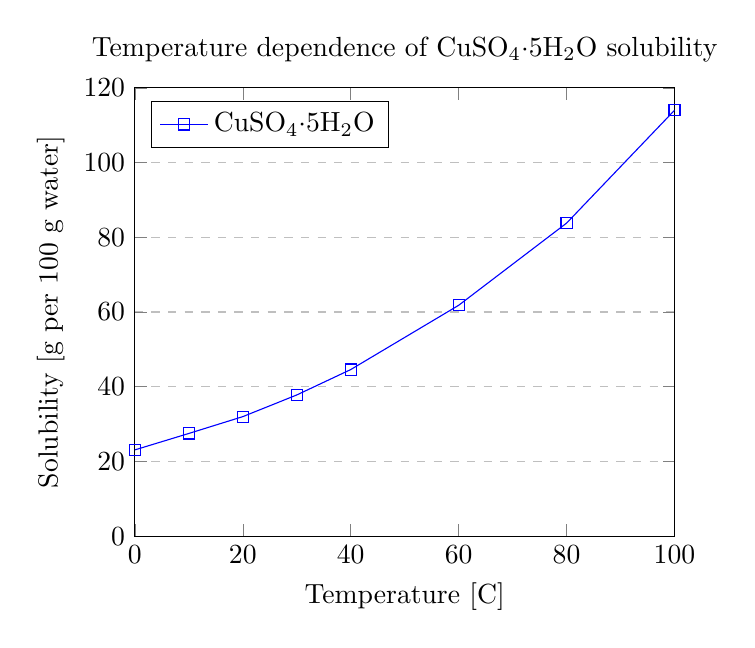
\begin{tikzpicture}
\begin{axis}[
    title={Temperature dependence of CuSO$_4\cdot$5H$_2$O solubility},
    xlabel={Temperature [C]},
    ylabel={Solubility [g per 100 g water]},
    xmin=0, xmax=100,
    ymin=0, ymax=120,
    xtick={0,20,40,60,80,100},
    ytick={0,20,40,60,80,100,120},
    legend pos=north west,
    ymajorgrids=true,
    grid style=dashed,
]
 
\addplot[
    color=blue,
    mark=square,
    ]
    coordinates {
    (0,23.1)(10,27.5)(20,32)(30,37.8)(40,44.6)(60,61.8)(80,83.8)(100,114)
    };
    \legend{CuSO$_4\cdot$5H$_2$O}
 
\end{axis}
\end{tikzpicture}







\bibliographystyle{plain}
\bibliography{LaTeX.bib}


%\item What \textbf{part} of the document is this? Should it have treated that sentence as our name? a title? the opening paragraph or abstract?



\end{document}
